\documentclass[dvipdfmx,a4paper]{jsarticle}
    \pagestyle{plain}
\usepackage{amsmath}
\usepackage{amsthm}
\usepackage{amssymb}
\usepackage{graphicx}
\usepackage{tikz}
\usepackage{tkz-euclide}
\usepackage{here}
\usepackage{cancel}

\usetikzlibrary{angles}
\usetikzlibrary{calc}

\newcommand{\R}{\mathbb{R}}
\newcommand{\C}{\mathbb{C}}
\newcommand{\Z}{\mathbb{Z}}
\newcommand{\N}{\mathbb{N}}
\newcommand{\Q}{\mathbb{Q}}
\newcommand{\Lra}{\Leftrightarrow}
\newcommand{\al}{\alpha}
\newcommand{\be}{\beta}
\newcommand{\ga}{\gamma}
\newcommand{\om}{\omega}
\newcommand{\De}{\Delta}
\newcommand{\oraw}{\overrightarrow}
\newcommand{\posv}[1]{\overrightarrow{\mathrm{#1}}}
\newcommand{\comb}[2]{{}_{#1}\mathrm{C}_{#2}}
\newcommand{\perm}[2]{{}_{#1}\mathrm{P}_{#2}}
\newcommand{\bs}{\backslash}
\newcommand{\2}{I\hspace{-1pt}I}
\newcommand{\3}{I\hspace{-1pt}I\hspace{-1pt}I}

\newtheorem{cs}{Case}
\newtheorem{cas}{Case}
\newtheorem{case}{Case}
\newtheorem{apf}{別解}
\newtheorem{anpf}{別解}
    
    % maketitle
    \title{2022年度京大数学(文系)の問題}
    \author{tt0801}
    \date{\today}
    
    \begin{document}
    \maketitle
    \section{大問1}
    $5.4 < \log_4 2022 < 5.5$であることを示せ. ただし, $0.301 < \log_{10} 2 < 0.3011$であることは用いてよい. 


    \section{大問2}
    下図の三角柱$\mathrm{ABC - DEF}$において, Aを始点として, 辺に沿って頂点を$n$回移動する. すなわち, 
    この移動経路
    \begin{equation*}
        \mathrm{
            P_0 \rightarrow P_1 \rightarrow P_2 \rightarrow \cdots 
            \rightarrow P_{n-1} \rightarrow P_n \quad (ただし P_0 = A)
        }
    \end{equation*}
    において, $\mathrm{P_0P_1, P_1P_2, \cdots, P_{n-1}P_n}$はすべて辺であるとする. また, 
    同じ頂点を何度通ってもよいものとする. このような移動経路で, 終点$\mathrm{P_n}$が
    A, B, Cのいずれかとなるものの総数$a_n$を求めよ. 

    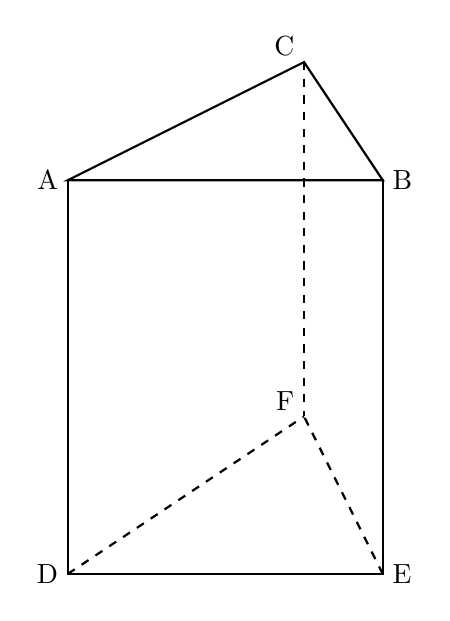
\begin{tikzpicture}
        % Draw the base square A - B - E - D
        \draw[thick] (0,0) -- (4,0) -- (4,-5) -- (0,-5) -- cycle;

        % Draw the top triangle A - C - B
        \draw[thick] (0,0) -- (3,1.5) -- (4,0) -- cycle;

        % Connect base to apex of the triangle C - F
        \draw[thick, dashed] (3,1.5) -- (3,-3);

        % Draw the diagonal lines of the base D - F, E - F
        \draw[thick, dashed] (0,-5) -- (3,-3);
        \draw[thick, dashed] (4,-5) -- (3,-3);

        % Label the points
        \node[anchor=east] at (0,0) {A};
        \node[anchor=west] at (4,0) {B};
        \node[anchor=east] at (3,1.7) {C};
        \node[anchor=east] at (0,-5) {D};
        \node[anchor=west] at (4,-5) {E};
        \node[anchor=east] at (3,-2.8) {F};
    \end{tikzpicture}

    \section{大問3}
    $xy$平面上の2直線$L_1, L_2$は直交し, 交点の$x$座標は$\dfrac{3}{2}$である. また, 
    $L_1, L_2$はともに曲線$C: y = \dfrac{x^2}{4}$に接している. 
    このとき, $L_1, L_2$および$C$で囲まれる図形の面積を求めよ. 

    \section{大問4}
    $a,b$を正の実数とする. 直線$L: ax+by=1$と曲線$y=-\dfrac{1}{x}$との2つの交点のうち, 
    $y$座標が正のものをP, 負のものをQとする. また, $L$と
    $x$軸の交点をRとし, $L$と$y$軸の交点をSとする. $a,b$が条件
    \begin{equation*}\mathrm{
        \dfrac{PQ}{RS} = \sqrt{2}
    }
    \end{equation*}
    を満たしながら動くとき, 線分PQの中点の軌跡を求めよ. 

    \section{大問5}
    四面体OABCが
    \begin{equation*}
        \mathrm{
            OA = 4,\ OB=AB=BC=3,\ OC=AC=2\sqrt{3}
        }
    \end{equation*}
    を満たしているとする. 点Pを辺BC上の点とし, $\triangle \mathrm{OAP}$の
    重心をGとする. このとき, 次の各問に答えよ. 
    \begin{itemize}
        \item [(1)] $\oraw{\mathrm{PG}} \perp \oraw{\mathrm{OA}}$を示せ. 
        \item [(2)] Pが辺BC上を動くとき, PGの最小値を求めよ. 
    \end{itemize}

    


\end{document}